%!TEX TS-program = xelatex
%!TEX encoding = UTF-8 Unicode

\documentclass[a4paper,11pt,twoside]{book}
\usepackage{upatras-thesis}


%
% These commands need to be defined in order to produce a correct and personalized document
%
\newcommand{\shortdoctitle}{Διπλωματική Εργασία}
\newcommand{\doctitle}{Τίτλος Εργασίας}
\newcommand{\docsubtitle}{Υπότιτλος εγγράφου}
\newcommand{\division}{Τομέας Φοιτητή}
\newcommand{\lab}{Εργαστήριο Εκπόνησης της Εργασίας}

\newcommand{\me}{Όνομα και Επώνυμο Φοιτητή}
\newcommand{\studnum}{Μητρώο Φοιτητή}
\newcommand{\keywords}{keyword1, keyword2,keyword3}
\newcommand{\monthyear}{Μήνας 201X}

\newcommand{\supname}{Ονοματεπώνυμο Επιβλέποντα}
\newcommand{\suptitle}{Βαθμίδα Επιβλέποντα}
\newcommand{\headofdivision}{Ονοματεπώνυμο Διεθυντή Τομέα}
\newcommand{\headofdivisiontitle}{Βαθμίδα Διευθυντή Τομέα}

\author{\me}


% PDF settings
%
\hypersetup
{
    pdfauthor={\me},
    pdftitle={\shortdoctitle},
    pdfsubject={\doctitle},
    pdfkeywords={\keywords}
}

\begin{document}


\pagenumbering{roman}
%set the number of sectioning levels that get number and appear in the contents
\setcounter{page}{3}

\begin{titlepage}
\begin{center}
% Upper part of the page
\textsc{\textbf{\large ΠΑΝΕΠΙΣΤΗΜΙΟ ΠΑΤΡΩΝ - ΠΟΛΥΤΕΧΝΙΚΗ ΣΧΟΛΗ}\\
\large ΤΜΗΜΑ ΗΛΕΚΤΡΟΛΟΓΩΝ ΜΗΧΑΝΙΚΩΝ\\ΚΑΙ ΤΕΧΝΟΛΟΓΙΑΣ ΥΠΟΛΟΓΙΣΤΩΝ}\\[0.5cm]


\includegraphics[width= \textwidth]{up_landscape}\\[0.5cm]  

\textsc{\Large τομέας: \division \\
εργαστήριο: \lab }\\[1cm]

\textsc{\uline{\LARGE{\shortdoctitle }}}\\ [0.5cm]
του φοιτητή του Τμήματος Ηλεκτρολόγων Μηχανικών και Τεχνολογίας\\
Υπολογιστών της Πολυτεχνικής Σχολής  του Πανεπιστημίου Πατρών\\[1cm]

\textsc{\LARGE \me }\\[0.5cm]
\textsc{\Large αριθμός μητρώου: \studnum}\\[1cm]

\uline{\large Θέμα}\\[0.5cm]
\textbf{\large \doctitle }\\[1cm]
\uline{\large Επιβλέπων}\\[0.5cm]
\large \suptitle \, \supname \\[1cm]
\large{Αριθμός Διπλωματικής Εργασίας: }\hspace{3cm}
\vfill
% Bottom of the page
\large{Πάτρα, \monthyear}
\end{center}
\end{titlepage}

\clearemptydoublepage

\pagestyle{empty}
\begin{center}
{\LARGE ΠΙΣΤΟΠΟΙΗΣΗ\\[1cm]}
\large Πιστοποιείται ότι η διπλωματική εργασία με θέμα\\[1cm]
\textbf{\large \doctitle }\\[1cm]
του φοιτητή του Τμήματος Ηλεκτρολόγων Μηχανικών και Τεχνολογίας Υπολογιστών\\[1.5cm]
\me \\[0.5cm]
(Α.Μ.: \studnum )\\[1.5cm]
παρουσιάτηκε δημόσια και εξετάστηκε στο τμήμα  Ηλεκτρολόγων Μηχανικών και Τεχνολογίας Υπολογιστών στις\\[1cm]
\Large{\_\_/\_\_/\_\_\_}\\[1.5cm]
\end{center}
\begin{minipage}{0.5\textwidth}
\begin{flushleft} \large
Ο Επιβλέπων\\[4cm]
\supname \\
\emph{\suptitle}
\end{flushleft}
\end{minipage}
\begin{minipage}{0.5\textwidth}
\begin{flushright} \large
Ο Διευθυντής του Τομέα\\[4cm]
\headofdivision\\
\emph{\headofdivisiontitle}
\end{flushright}
\end{minipage}

\clearemptydoublepage

\pagestyle{empty}
\begin{center}
\Large{Στοιχεία διπλωματικής εργασίας}\\[1cm]
{\large Θέμα:}
\textbf{\large \doctitle}\\[1cm]
\large {Φοιτητής: \textbf{\me}\\[1cm]
\large{Ομάδα επίβλεψης}\\
\textbf{\suptitle \, \supname}\\
\textbf{Βαθμίδα και Ονοματεπώνυμο Συνεπιβλέποντα}\\
\textbf{Ονοματεπώνυμο Διδακτορικού Φοιτητή}\\[1cm]
Εργαστήρια\\
\lab \\[1cm]
Περίοδος εκπόνησης της εργασίας:\\ Μήνας Έτος - Μήνας Έτος\\[1cm]
Η εργασία αυτή γράφτηκε στο \XeLaTeX{} και χρησιμοποιήθηκε η γραμματοσειρά GFS Didot του Greek Font Society.}
\end{center}

\clearemptydoublepage

\pagestyle{plain}
\begin{center}
{\LARGE Περίληψη}\\[1cm]
\end{center}

\lettrine[findent=2pt]{\fbox{\textbf{H}}}{ } εργασία αυτή ασχολείται με ένα ιδιαίτερα ενδιαφέρον ζήτημα στο χώρο της επεξεργασίας σημάτων και εικόνων, την ανάλυση (\emph{resolution}). Παρόλο που σήμερα στον κόσμο μας έχουμε καταφέρει να δημιουργήσουμε συσκευές με μεγάλη ευαισθησία καταγραφής, μεγάλο χώρο αποθήκευσης καθώς και υψηλούς ρυθμούς μετάδοσης και επεξεργασίας δεδομένων, εντούτοις υπάρχουν εφαρμογές όπου η φύση τους είναι τέτοια που δε μας επιτρέπει να επωφεληθούμε σε μεγάλο βαθμό από την πρόοδο που έχει σημειωθεί. Μια τέτοια εφαρμογή είναι οι θερμικές εικόνες και θα δούμε στη συνέχεια της εργασίας τους λόγους εκείνους που την καθιστούν ``ιδιαίτερη".


\clearemptydoublepage

\begin{center}
{\LARGE Ευχαριστίες}\\[1cm]
\end{center}

\lettrine[findent=2pt]{\fbox{\textbf{Ό}}}{σο} κι αν φαίνεται σαν ατομική δουλειά η παρούσα εργασία, στην πραγματικότητα βοήθησαν αρκετοί άνθρωποι (ο καθένας με το δικό του τρόπο) για να ολοκληρωθεί. 

\clearemptydoublepage

\pagestyle{fancy}

\tableofcontents
%\mainmatter % book mode only
\clearemptydoublepage

\pagenumbering{arabic}
\setcounter{page}{1}

%!TEX root = ../main.tex

\chapter*{Εισαγωγή}
\markboth{Εισαγωγη}{}
%\vspace{-1.3in}
\lettrine[findent=2pt]{\fbox{\textbf{Η}}}{εργασια} αυτή έχει γίνει προσπάθεια να γραφεί σε ανεξάρτητα κεφάλαια, τα οποία θα δώσουν στον αναγνώστη τις απαιτούμενες γνώσεις ώστε να καταλάβει σε βάθος τις τεχνικές που χρησιμοποιούνται. Σε κάθε κεφάλαιο γίνεται αναλυτική παρουσίαση των τεχνικών καθώς και του υπόβαθρου που πρέπει να έχει κάποιος ώστε τις κατανοήσει, ωστόσο θεωρείται πως ο αναγνώστης έχει ήδη κάποιες γνώσεις στο χώρο της επεξεργασίας σήματος και εικόνας. Έτσι, βασικές έννοιες και μηχανισμοί της ανωτέρω περιοχής θα θεωρούνται δεδομένοι και δε θα γίνει κάποια ανάλυσή τους στο κείμενο αυτό, εκτός αν κρίνεται απαραίτητο.

\clearemptydoublepage

\chapter{Οι θερμικές εικόνες}\label{ch:chap1}
%!TEX root = ../main.tex



\section{Η υπέρυθρη ακτινοβολία}

\begin{figure}
  \centering
  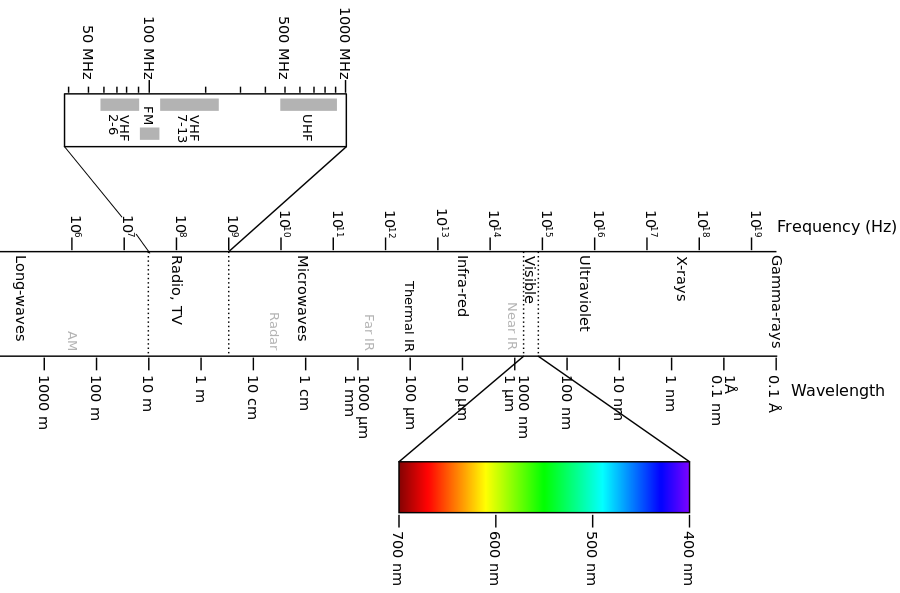
\includegraphics[width=\textwidth]{spectrum}
  \caption{Το φάσμα της Ηλεκτρομαγνητικής Ακτινοβολίας}
  \label{fig:spectrum}
\end{figure}

\lettrine[findent=2pt]{\fbox{\textbf{Ό}}}{πως} γνωρίζουμε από την επιστήμη της Φυσικής, όταν ένα σώμα ζεσταθεί αρκετά (π.χ. > 100 \degree C) αρχίζει και εκπέμπει ακτινοβολία και στο οπτικό φάσμα (πέραν του υπέρυθρου), ενώ αποκτά ταυτόχρονα μια ερυθρή όψη. Κατά το φαινόμενο αυτό, η ακτινοβολια που εκπέμπεται ανήκει τόσο στο υπέρυθρο, όσο και στο ορατό φάσμα της ηλεκτρομαγνητικής ακτινοβολίας και μάλιστα το χρώμα που αποκτά το σώμα συνδέεται άμεσα με τη θερμοκρασία στην οποία βρίσκεται. Οι περιοχές της υπέρυθρης και ορατής ακτινοβολίας, καταλαμβάνουν τις ζώνες $1mm - 700nm$ και $700nm - 390nm$ αντίστοιχα, όπως φαίνεται και στο σχήμα \ref{fig:spectrum}.


\clearemptydoublepage

\chapter{Η ανάλυση}\label{ch:chap2}
%!TEX root = ../main.tex



\section{Η έννοια της ανάλυσης}

\lettrine[findent=2pt]{\fbox{\textbf{Κ}}}{ατά} την αποτύπωση οποιουδήποτε αναλογικού σήματος $S(t)$ σε ψηφιακή μορφή $S_i$, πραγματοποιείται μια διαδικασία που ονομάζεται \emph{δειγματοληψία (sampling)} κατά την οποία ένα συνεχές σήμα γίνεται διακριτό και στη συνέχεια εφαρμόζουμε \emph{κβαντισμό} στις τιμές του, για να περάσουμε σε ψηφιακή αναπαράσταση. Όπως φαίνεται και στο σχήμα \ref{fig:sampling}, σε διακριτές χρονικές στιγμές λαμβάνουμε την τιμή του αναλογικού σήματος (μέσω ενός μετατροπέα Αναλογικού σε Ψηφιακό (ADC)) κι έτσι δημιουργούμε μια σειρά από τιμές (\emph{δείγματα}) τα οποία έχουν συγκεκριμένη και σταθερή χρονική απόσταση $T_s$. Η χρονική απόσταση έχει νόημα μόνο ως προς το αναλογικό σήμα, ενώ στην ψηφιακή μορφή των δειγμάτων αναφερόμαστε σε αυτά με ένα δείκτη $n$ και μεταξύ αναλογικού και ψηφιακού σήματος ισχύει ότι $S_i=S(nT_s)$.
\begin{figure}[h]
  \centering
  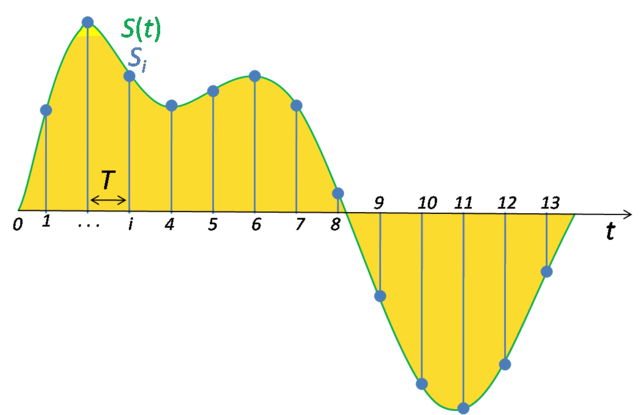
\includegraphics[width=0.6\textwidth]{Signal_Sampling}
  \caption{Δειγματοληψία ενός αναλογικού σήματος}
  \label{fig:sampling}
\end{figure}
Κατά τη δειγματοληψία ``χάνουμε'' αρκετή από την πληροφορία που περιέχει το αναλογικό σήμα, καθώς οι τιμές που βρίσκονται μεταξύ των διαστημάτων $T_s$ όπου λαμβάνουμε δείγματα δε λαμβάνονται υπόψη. Ακόμη, λόγω της πεπερασμένης ακρίβειας των ψηφιακών συστημάτων για αναπαράσταση αριθμών, η τιμή που έχει το σήμα στρογγυλοποιείται στην πλησιέστερη (είτε μεγαλύτερη είτε μικρότερη) τιμή που μπορεί να αναπαραστήσει το σύστημά μας.

Όπως γίνεται αντιληπτό, σε πολλές των περιπτώσεων η δειγματοληψία μπορεί να έχει καταστροφικές συνέπειες για το αναλογικό σήμα. Ωστόσο, υπό προϋποθέσεις, μπορεί να είναι αντιστρεπτή διαδικασία -- μπορούμε δηλαδή από τα δείγματα που έχουμε λάβει να επιστρέψουμε στην αναλογική μορφή του σήματος. Οι προϋποθέσεις αυτές ορίζονται από το θεώρημα \emph{Shannon-Nyquist} (\ref{thrm:shannon-nyquist}), ως:
\\
\begin{theorem}[Shannon-Nyquist]
	\label{thrm:shannon-nyquist}
	Ένα σήμα με μέγιστη συχνότητα $f_{max}$ μπορεί να ανακτηθεί από τα δείγματά του, αν αυτά ληφθούν με συχνότητα $f_s>2f_{max}$, ή αλλιώς με περίοδο $T_s<\frac{1}{2f_{max}}$. \cite{proakis_sampling}
\end{theorem}
\clearemptydoublepage

\chapter{Super Resolution μέσω Image Registration}\label{ch:chap3}
%!TEX root = ../main.tex



\section{Μοντελοποίηση προβλήματος}

\lettrine[findent=2pt]{\fbox{\textbf{Π}}}{ριν} δούμε στην πράξη πώς λειτουργούν οι τεχνικές super resolution θα πρέπει να περιγράψουμε το πρόβλημα με το οποίο θα δουλέψουμε με μαθηματικούς όρους. Η μοντελοποίηση αυτή θα μας επιτρέψει να χρησιμοποιήσουμε μαθηματικά εργαλεία και τεχνικές και να ορίσουμε σε μια αυστηρή ``γλώσσα'' (αυτή των μαθηματικών) τις λειτουργίες που επιτελούνται από κάθε μέθοδο, ούτως ώστε να πετύχουμε το τελικό αποτέλεσμα.

Ξεκινώντας, θα πρέπει να περιγράψουμε τον τρόπο με τον οποίο λαμβάνουμε εικόνες χαμηλής ανάλυσης από μια φυσική σκηνή μέσω μιας κάμερας. Η κάμερα σαν όργανο καταγραφής εισάγει κάποιες ατέλειες, όπως είδαμε στο προηγούμενο κεφάλαιο. Τέτοιες ατέλειες μπορεί να είναι σφάλματα καταγραφής από τον αισθητήρα της κάμερας, θόλωμα λόγω αστοχιών των οπτικών στοιχείων κλπ. Επιπλέον, αν λάβουμε διαδοχικές εικόνες μιας φυσικής σκηνής, οι εικόνες αυτές περιμένουμε να έχουν κάποιες μετατοπίσεις ως προς αυτό που απεικονίζουν. Οι μετατοπίσεις αυτές μπορεί να οφείλονται είτε στον άνθρώπινο παράγοντα (που χειρίζεται την κάμερα) είτε στο αντικείμενο της φυσικής σκηνής που μπορεί να μην είναι σταθερό. Στην εικόνα που λαμβάνεται τελικά, λαμβάνονται δείγματα σε χαμηλή χωρική συχνότητα και λόγω ατελειών του οργάνου μπορεί να έχουμε και παρουσία θορύβου. Για μια εικόνα υψηλής ανάλυσης $\bm{X}$ (την οποία θα προσπαθήσουμε να ανακατασκευάσουμε), μπορούμε να αναπτύξουμε το παραπάνω μοντέλο ως εξής:
\begin{equation} \label{eq:hrmodel}
\bm{Y}_i=\bm{S}_i\bm{T}_i\bm{H}_i\bm{X}+\bm{n}_i
\end{equation}
όπου ορίζουμε για την i-οστή εικόνα χαμηλής ανάλυσης $\bm{Y}_i$ τους τελεστές που ενεργούν στην $\bm{X}$ : 
\begin{itemize}
	\item $\bm{S}_{i}$ για υποδειγματοληψία, 
	\item $\bm{T}_{i}$ για μετατόπιση, 
	\item $\bm{H}_{i}$ για θόλωμα (blurring), 
	\item $\bm{n_{i}}$ για προσθετικό θόρυβο.
\end{itemize}
Οι υποθέσεις που κάνουμε για το παραπάνω πρόβλημα είναι ότι το blurring είναι ίδιο σε όλο το χώρο και είναι γνωστό στον αλγόριθμο super resolution, ο θόρυβος είναι λευκός Gaussian με την ίδια διασπορά σε όλες τις εικόνες χαμηλής ανάλυσης και ότι ο γεωμετρικός μετασχηματισμός αφορά μόνο την καθολική μετατόπιση. 

 Στην περίπτωση που θεωρήσουμε αμελητέο θόρυβο και θόλωμα, τα παραπάνω βήματα αρκούν για να υπολογίσουμε την εικόνα υψηλής ανάλυσης $\bm{X}$, την οποία λαμβάνουμε σαν αποτέλεσμα του αλγορίθμου.

\begin{algorithm}

 \KwData{$\bm{dx}$, $\bm{dy}$, $\bm{Y}_i$, $N$, $W$, $\bm{H}$, $S$}
 \KwOut{High resolution reconstructed $\bm{X}$}
 $\bm{X} \gets 0$\; 
 \For{$n \gets 1$ \textbf{to} $N$}{
 	$\bm{\tilde{Y}} \gets \bm{Y}_i$\;
    $\bm{i} \gets 1:W/S$\;
    $\bm{j} \gets 1:H/S$\;
    $\bm{px}=\bm{i}*S+\bm{dx}_n$\;
    $\bm{py}=\bm{j}*S+\bm{dy}_n$\;
    $\bm{X}_{px,py}=\bm{\tilde{Y}}_{i,j}$\;
    }
    %\vspace{-1.5em}
 \caption{Ανακατασκευή shift-add fusion}\label{algo:sr_fusion}
\end{algorithm}

Συγκρίνοντας τη μέθοδο αυτή με την ανακατασκευή μέσω του μετασχηματισμού Fourier, παρατηρούμε την απλότητα και την αποδοτικότητά της καθώς βρίσκει την εικόνα υψηλής ανάλυσης μόνο με μετακινήσεις pixel. 
\clearemptydoublepage

%!TEX root = ./main.tex

\begin{thebibliography}{99}

\bibitem{c1} S. C. Park, M. K. Park, and M. G. Kang, “Super-resolution image reconstruction:
A technical overview,” IEEE Signal Processing Magazine, vol. 20, no. 3, pp. 21–36,
May 2003.
\bibitem{keren} D. Keren, S. Peleg, and R. Brada, “Image sequence enhancement using subpixel
displacements,” in IEEE Computer Society Conference on Computer Vision and
Pattern Recognition, June 1988, pp. 742–746.
\bibitem{hardie} R. Hardie, K. Barnard, and E. Armstrong, “Joint MAP registration and high resolution image estimation using a sequence of undersampled images,” IEEE Transactions on Image Processing, vol. 6, no. 12, pp. 1621–1633, December 1997.
\bibitem{patti} A. Patti, M. Sezan, and A. Tekalp, “High-resolution image reconstruction from
a low-resolution image sequence in the presence of time-varying motion blur,” in
Proceedings of the IEEE International Conference on Image Processing, Austin,
TX, vol. 1, 1994, pp. 343–347.
\bibitem{hardie2} R. C. Hardie, K. J. Barnard, J. G. Bognar, E. E. Armstrong, and E. A. Watson, “High resolution image reconstruction from a sequence of rotated and translated
frames and its application to an infrared imaging system,” Optical Engineering,
vol. 37, no. 1, pp. 247–260, January 1998.
\bibitem{alam} M. S. Alam, J. G. Bognar, R. C. Hardie, and B. J. Yasuda, “Infrared image registration and high-resolution reconstruction using multiple translationally shifted aliased video frames,” IEEE Transactions on Instrumentation and Measurement, vol. 49,
no. 5, pp. 923–915, October 2000.
\bibitem{tsai} R. Y. Tsai and T. S. Huang, “Multiframe image restoration and registration,” in Advances in Computer Vision and Image Processing: Image Reconstruction from Incomplete Observations, T. S. Huang, Ed., vol. 1. London: JAI Press, 1984, pp. 317–339.
\bibitem{kim} N. K. Bose, H. C. Kim, and H. M. Valenzuela, “Recursive total least squares algorithm for image reconstruction from noisy undersampled frames,” Multidimensional Systems and Signal Processing, vol. 4, no. 3, pp. 253–268, July 1993.
\bibitem{yang} J. Yang, J. Wright, T. Huang, and Yi Ma. Image super-resolution via sparse representation. IEEE Transactions on Image Processing (TIP), vol. 19, issue 11, 2010.
\bibitem{ransac} Martin A. Fischler and Robert C. Bolles (June 1981). “Random Sample Consensus: A Paradigm for Model Fitting with Applications to Image Analysis and Automated Cartography”. Comm. of the ACM 24 (6): 381–395
\bibitem{wired_ff_algo} Jordan Ellenberg, ”Fill in the Blanks: Using Math to Turn Lo-Res Datasets Into Hi-Res Samples”, 22 February 2010, Wired Magazine \url{http://www.wired.com/2010/02/ff_algorithm/}
\bibitem{incoherence} D.L. Donoho and X. Huo, “Uncertainty principles and ideal atomic decomposition,” IEEE Trans. Inform. Theory, vol. 47, no. 7, pp. 2845–2862, Nov. 2001.
\bibitem{candes} E. Candes, “Compressive sensing,” in Proceedings of the International Congress of Mathematicians, vol. 3, pp. 1433–1452, 2006.
\bibitem{donoho} D. L. Donoho, “Compressed sensing,” IEEE Transactions on Information Theory, vol. 52, no. 4, pp. 1289–1306, 2006.
\bibitem{proakis_sampling} John G. Proakis, Dimitris G. Manolakis , “Digital Signal Processing - Principles, Algorithms, Implementations” 4th edition (Pearson International Edition), Pearson Education, Chapter 1.4.2: The Sampling Theorem 
\bibitem{gonzalez_2d_fft} Rafael C. Gonzalez, Richard E. Woods , “Digital Image Processing” 3rd edition (Pearson International Edition), Pearson Education, Chapter 1.4.2: The 2D Discrete Fourier Transform and its Inverse
\bibitem{shift_add_fusion} S. Farsiu, M. Elad, P. Milanfar, “Fast and Robust Multiframe Super Resolution” IEEE Transactions on Image Processing, vol. 13, no. 10, October 2004
\bibitem{imregintro} ”Image Registration", in Wikipedia: The Free Encyclopedia; (Wikimedia Foundation Inc., updated 2 December 2014, 15:50 UTC) \url{http://en.wikipedia.org/wiki/Image_registration}
\bibitem{cs_intro} M. Davenport, M. Duarte, Y. Eldar, G. Kutyniok, ”Introduction to Compressed Sensing”, Stanford University - Department of Statistics
\bibitem{convexmin} F. Bach, R. Jenatton, J. Mairal, G. Obozinski, ”Convex Optimization with Sparsity-Inducing Norms”, Institut National de Recherche en Informatique et en Automatique (INRIA)
\bibitem{red_dict} H. Rauhut, K. Schnass, and P. Vandergheynst, “Compressed sensing and redundant dictionaries,” IEEE Transactions on Information Theory, vol. 54, no. 5, May 2008.
\bibitem{denoising_dict} M. Elad and M. Aharon, “Image denoising via sparse and redundant representations over learned dictionaries,” IEEE Transactions on Image Processing, vol. 15, pp. 3736–3745, 2006.
\bibitem{im_vid_rest} J. Mairal, G. Sapiro, and M. Elad, “Learning multiscale sparse representations for image and video restoration,” Multiscale Modeling and Simulation, vol. 7, pp. 214–241, 2008.
\bibitem{ksvd_dict} M. Aharon, M. Elad, and A. Bruckstein, “K-SVD: An algorithm for designing overcomplete dictionaries for sparse representation,” IEEE Transactions on Signal Processing, vol. 54, no. 11, pp. 4311–4322, Nov. 2006.
\bibitem{sparse_coding_dict} H. Lee, A. Battle, R. Raina, and A. Y. Ng, “Efficient sparse coding algorithms,” in Advances in Neural Information Processing Systems (NIPS), pp. 801–808, 2007.
\bibitem{human_sparse} B. Olshausen and D. Field, “Sparse coding with an overcomplete basis set: A strategy employed by V1?,” Vision Research, vol. 37, no. 23, pp. 3311–3325, 1997.
\bibitem{nphard} ”NP-hard", in Wikipedia: The Free Encyclopedia; (Wikimedia Foundation Inc., updated 9 April 2015, 15:30 UTC) \url{http://en.wikipedia.org/wiki/NP-hard}
\bibitem{nphard1} D. L. Donoho, “For most large underdetermined systems of linear equations, the minimal $l_1$-norm solution is also the sparsest solution,” Communications on Pure and Applied Mathematics, vol. 59, no. 6, pp. 797–829, 2006.
\bibitem{nphard2} “For most large underdetermined systems of linear equations, the minimal $l_1$-norm near-solution approximates the sparsest near-solution,” Communications on Pure and Applied Mathematics, vol. 59, no. 7, pp. 907–934, 2006.
\bibitem{lasso} R. Tibshirani, “Regression shrinkage and selection via the lasso,” Jour- nal of Royal Statistical Society, Series B, vol. 58, no. 1, 1996.
\bibitem{dict_training} Jianchao Yang, Zhaowen Wang, Zhe Lin, and Thomas Huang. Coupled dictionary training for image super-resolution. IEEE Transactions on Image Processing (TIP), vol. 21, issue 8, pages 3467-3478, 2012.
\bibitem{srexample} W. T. Freeman, T. R. Jones, and E. C. Pasztor, “Example-based superresolution,” IEEE Computer Graphics and Applications, vol. 22, pp. 56–65, 2002.
\bibitem{lowlevel} W. T. Freeman, E. C. Pasztor, and O. T. Carmichael, “Learning low-level vision,” International Journal of Computer Vision, vol. 40, no. 1, pp. 25–47, 2000.
\bibitem{sr_neigh} H. Chang, D.-Y. Yeung, and Y. Xiong, “Super-resolution through neighbor embedding,” in IEEE Conference on Computer Vision and Pattern Classifi- cation (CVPR), vol. 1, pp. 275–282, 2004.
\bibitem{imhal} J. Sun, N. N. Zheng, H. Tao, and H. Shum, “Image hallucination with primal sketch priors,” in IEEE Conference on Computer Vision and Pattern Recognition (CVPR), vol. 2, 2003, pp. 729–736.
\bibitem{imfill} imfill, Image Processing Toolbox Documentation, MathWorks \\ \url{http://www.mathworks.com/help/images/ref/imfill.html}
\bibitem{imresize} imresize, Image Processing Toolbox Documentation, MathWorks \\ \url{http://www.mathworks.com/help/images/ref/imresize.html}
\bibitem{k-term} A. Cohen, W. Dahmen, R. DeVorce, "Compressed sensing and best k-term approximation", in the Journal of the American Mathematical Society, vol. 22, pp. 211-231 , 2009.




\end{thebibliography}
\clearemptydoublepage

\pagestyle{empty}

\vspace*{\fill}
\hline
\begin{flushleft}
	Πανεπιστήμιο Πατρών, Πολυτεχνική Σχολή \\
	Τμήμα Ηλεκτρολόγων Μηχανικών και Τεχνολογίας Υπολογιστών \\
	\me \\
	© \monthyear \ -- Με την επιφύλαξη παντός δικαιώματος.\\
\end{flushleft}
\hline


\end{document}
